\section{HalfCheetah}
The learning curve for a policy trained on the \texttt{HalfCheetah-v1}
environment is given in \figref{cheetah}. The policy obtained a score of 150
around iteration 85, peaked at an average score of around 160, and ended after
100 iterations on a score of around 150. The script used to run the experiment
is given in \figref{cheetah-script}. I used a very simple neural network with 2
hidden layers with 32 units each, reward-to-go, no baseline, and a learning
rate of 0.02. Most notably, I used a very large batch size of 50,000.

\begin{figure}[h]
  \centering
  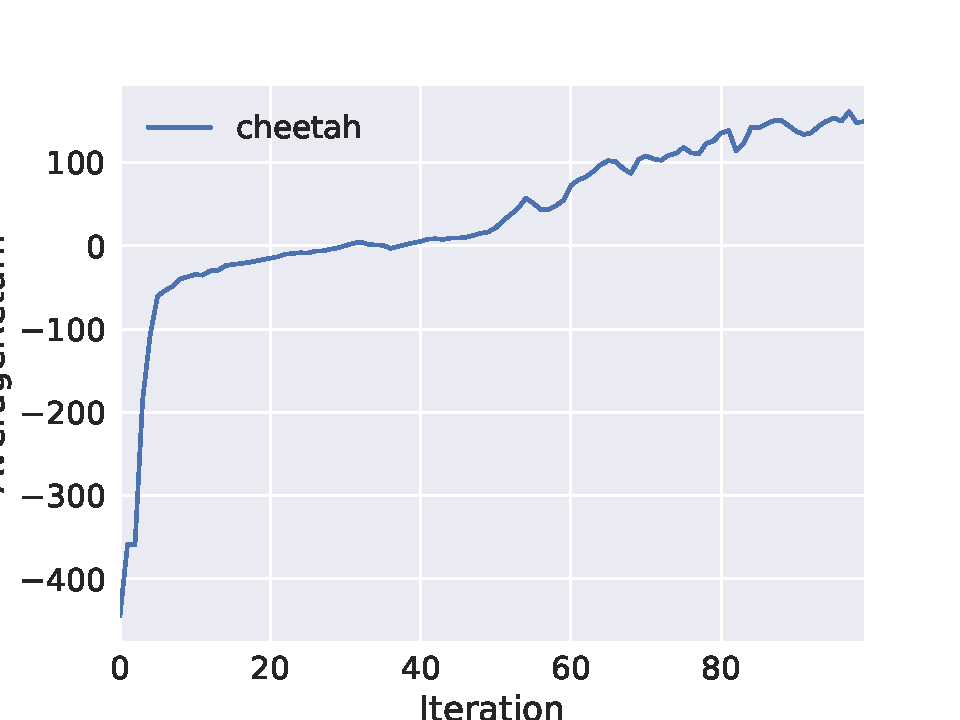
\includegraphics[width=\textwidth]{cheetah.pdf}
  \caption{Learning curve for \texttt{HalfCheetah-v1} environment.}
  \label{fig:cheetah}
\end{figure}

\begin{figure}
  \centering
  \footnotesize
  \begin{Verbatim}[gobble=4]
    #! /usr/bin/env bash

    set -euo pipefail

    main() {
        fixed_flags="-ep 150 --discount 0.9 -n 100"
        python train_pg.py \
            HalfCheetah-v1 \
            $fixed_flags \
            --verbose \
            --n_layers 2 \
            --size 32 \
            --seed 3 \
            -b 50000 \
            -e 1 \
            --learning_rate 0.02 \
            -rtg \
            --exp_name cheetah
    }

    main
  \end{Verbatim}
  \caption{Script use to run \texttt{HalfCheetah-v1} experiment.}
  \label{fig:cheetah-script}
\end{figure}
